\section{Deep Learning Approach} \label{sec:build4}

Artificial Neural Networks was an idea conceived  in the 1960s to mimic the functions of the human brain in the way it absorbs information and learns from it. in order to  convert the whole notion into reality it took a lot more time than expected. The primary reason behind the delay is that back then, the computers were not powerful enough, the other reasons being the researchers were not totally aware of the problem. Then in 1986, eminent neural network researcher and computer scientist Dr. Geoffrey Hinton came up with the idea of backpropagation[hinton paper] where a Deep Neural Network could be trained discriminatively and the weight updates can be done via stochastic gradient descentusing the following equation.

\begin{center}
	$w_{ij}(t+1) = w_{ij}(t) + \eta \frac{\partial C}{\partial w_{ij}}$
\end{center}
where $\eta$ s the learning rate, C is the cost function. The choice of the cost function depends on factors such as learning type whether it be supervised, unsupervised or reinforcement learning. 

The ability of multi-layer backpropagation[hinton backpropagation paper] networks has enabled the machines to learn complex high-dimensional non-linear mappings from large collections of example data which makes it obvious for visual recognition. In this method, rather than hand-crafting the various features, a raw image is first convoluted with a filter to find various feature maps. The feature maps are then connected together to form a fully-connected layer, the input of one layer is fed as the output of the next layer to create a deep network. The whole process rely on backpropagation to turn the first few layers into an appropriate feature extractor. Deep learning has achieved a lot of successes in the past for character recognition, digit recognition and recent works show that it is being applied to most topics of image representation and learning purposes. Just recently it has been applied to Face Recognition by training with lots of face image data and tremendous success has been reported[deep face paper].

The whole process of deep Convolutional Neural Networks(CNN)[leCunn paper] is very complex and requires a lot of computation to train and as a matter of fact, parallel computing is being brought forward to decrease the training time. The fully connected layer has several hundred hidden units and each of these units have specific weights assigned to them with the help of the back-propagation algorithm. Overfitting occurs if training data is scarce. Before being connected to the fully-connected neural network, the images need to be size normalized and centered in input fields. CNNs force the extraction of certain local features rather than global features which are obtained by hand-crafted feature extractors.

Deep Learning research stopped even after all these breakthroughs because the computers took a lot of time to train the large neural nets and at the same time a lot of image data was also not available. Researchers thought that it is better to go ahead with hand-crafted feature extractors which were giving better results at that time and took less time for computation. In 2006, Geoffrey Hinton and Ruslan Salakhuditnov worked on reducing the dimension of the data with neural networks in thier paper[DBN paper]. Since then a lot of work has been done as computers have become powerful with the advent of modern parallel processing algorithms. One of the major breakthroughs came in 2012, when Alex Krizhevsky[AlexNet paper] build a huge neural network by training 15 million images and then using Deep CNN they got one of the best result in the ImageNet competition for Image recognition and got a result which  was nearly 11 p.c. better than the second best approach which was done with SIFT + Fisher Vectors [Fei Fei Li paper]. Since then in the last 4 years quite a good amount of work has been done in this field. Several deep learning frameworks have been designed by researchers for researchers to move the work ahead - Some of the famous Frameworks being Caffe[Caffe Paper] by University of California, Berkeley, Theano[Theano Paper] by University de Montreal, TensorFlow[TF Paper] by Google, Torch[Torch Paper] and many others.

In our project we have used the Caffe Deep Learning Framework[Caffe Paper] for our purposes. The reason we choose Caffe is being described below:

Caffe provides multimedia scientists and practitioners with a clean and modifiable framework for state of the art deep learning algorithms. It has a big collection of reference CNN models, it is licensed with BSD and is written in C++ and Python. Caffe can process upto 40 million images a day on a single NVIDIA K40. Caffe is maintained by Berkeley Vision and Learning Center(BVLC). Caffe makes it easy for users to build CNNs in their .prototxt file and also has several functions to draw networks and optimize them. It provides Pre-Trained models which is not provided by many of its competetitors. Caffe stores nd communicates data in 4-arrays called blobs for faster processing. Blobs provide a unified memory interface, holding batches of images , parameters or parameters updates. Blobs conceal the mental and mental overhead of mixed CPU/GPU operation by synchronizing from the CPU host to the CPU device as needed. 

Caffe Neural Network Model prototxt format is being shown below:

\begin{lstlisting}% Start your code-block
name: "LeNet"
layer {
  name: "data"
  type: "Input"
  top: "data"
  input_param { shape: { dim: 64 dim: 1 dim: 28 dim: 28 } }
}
layer {
  name: "conv1"
  type: "Convolution"
  bottom: "data"
  top: "conv1"
  param {
    lr_mult: 1
  }
  param {
    lr_mult: 2
  }
  convolution_param {
    num_output: 20
    kernel_size: 5
    stride: 1
    weight_filler {
      type: "xavier"
    }
    bias_filler {
      type: "constant"
    }
  }
}
layer {
  name: "pool1"
  type: "Pooling"
  bottom: "conv1"
  top: "pool1"
  pooling_param {
    pool: MAX
    kernel_size: 2
    stride: 2
  }
}
layer {
  name: "conv2"
  type: "Convolution"
  bottom: "pool1"
  top: "conv2"
  param {
    lr_mult: 1
  }
  param {
    lr_mult: 2
  }
  convolution_param {
    num_output: 50
    kernel_size: 5
    stride: 1
    weight_filler {
      type: "xavier"
    }
    bias_filler {
      type: "constant"
    }
  }
}
layer {
  name: "pool2"
  type: "Pooling"
  bottom: "conv2"
  top: "pool2"
  pooling_param {
    pool: MAX
    kernel_size: 2
    stride: 2
  }
}
layer {
  name: "ip1"
  type: "InnerProduct"
  bottom: "pool2"
  top: "ip1"
  param {
    lr_mult: 1
  }
  param {
    lr_mult: 2
  }
  inner_product_param {
    num_output: 500
    weight_filler {
      type: "xavier"
    }
    bias_filler {
      type: "constant"
    }
  }
}
layer {
  name: "relu1"
  type: "ReLU"
  bottom: "ip1"
  top: "ip1"
}
layer {
  name: "ip2"
  type: "InnerProduct"
  bottom: "ip1"
  top: "ip2"
  param {
    lr_mult: 1
  }
  param {
    lr_mult: 2
  }
  inner_product_param {
    num_output: 10
    weight_filler {
      type: "xavier"
    }
    bias_filler {
      type: "constant"
    }
  }
}
layer {
  name: "prob"
  type: "Softmax"
  bottom: "ip2"
  top: "prob"
}
\end{lstlisting}

\begin{figure}[t]
	\DeclareGraphicsExtensions{.pdf,.png,.jpg}
	\begin{center}
		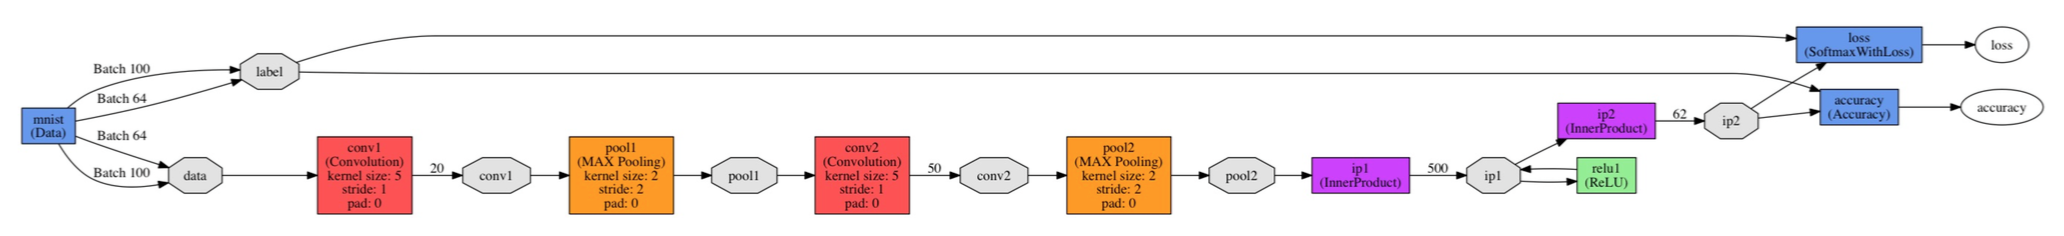
\includegraphics[width=\textwidth]{Figures/Figure18}
	\end{center}
	\caption{LeNet Network Diagram}
	\label{fig:Figure18}
\end{figure}
